\section{fulibWorkflows}\label{sec:fulibworkflows2}
\textit{fulibWorkflows} ist eine Java-Bibliothek, welche Workflow Beschreibungen als Eingabe bekommt, diese Eingabe
selbst parst und daraus HTML-/FXML-Mockups, Objektdiagramme und Klassendiagramme generiert.
Das Parsen wird über einen von Antlr generierten Parser übernommen, hierzu wird in Kapitel~\ref{subsec:antlr-grammatik} genauer auf
die zugrundeliegende Grammatik eingegangen.
Zudem wird auf die Limitationen des Parsers und der generierten Mockups eingegangen.

\subsection{Workflow-Format}\label{subsec:workflow-format}
Bevor in Kapitel~\ref{subsec:datenmodell} auf den Parser und das Datenmodell einer Workflow-Beschreibung eingegangen wird,
ist es nötig das Format in welcher ein Workflow beschrieben werden muss, näher zu beleuchten.
Die Grundlage des Formats bildet~\ac{YAML}.
Wobei das Format durch ein JSON-Schema stark begrenzt ist.
Näheres zu den Beschränkungen der Syntax wird in Kapitel~\ref{subsec:schema} erklärt.

\begin{listing}[!ht]
    \inputminted{yaml}{listings/3.1.1/allNotes.es.yaml}
    \caption{Beispiel aller vorhandenen Post-its\textsuperscript{\textregistered}}
    \label{listing:workflowNotes}
\end{listing}

In Listing~\ref{listing:workflowNotes} sind alle möglichen Post-its\textsuperscript{\textregistered} aufgelistet.
Im weiteren Verlauf wird für einen Post-it\textsuperscript{\textregistered} das Wort Zettel verwendet, da es sich bei jedem Element in der Beschreibung um einen einzelnen Zettel aus dem Event Storming handelt.
Als Beispiel für einen Workflow ist hierbei die Registrierung eines neuen Benutzenden auf einer Webseite in vereinfachter Form dargestellt.
Folgend werden alle verwendbaren Zettel aus der aktuellen Version, v0.4.0, von fulibWorkflows aufgelistet und deren Funktion erläutert.

\largerText{workflow}

Zum Darstellen eines oder mehrerer Workflows benötigt es den \textit{workflow}-Zettel.
Diesem kann nur ein Name zugeordnet werden, allerdings werden alle weiteren Zettel unter einem workflow-Zettel ebendiesem Workflow zugewiesen.
Pro Workflow-Beschreibung benötigt es somit mindestens einen workflow-Zettel.
Im vorherigen Beispiel gibt es einen Workflow mit dem Namen~\textit{User Registration}.

\largerText{service}

Durch den \textit{service}-Zettel werden Services bereitgestellt.
Diese sind einzig zur Strukturierung des Workflows und dem später daraus entstehenden~\ac{ES}-Board da.
Hiermit kann erreicht werden, dass die nach einem service-Zettel folgenden Zettel von dem vorherigen Service ausgeführt werden.
Im Beispiel aus Listing~\ref{listing:workflowNotes} gibt es nur einen Service, dieser kümmert sich um die Nutzerverwaltung, daher
stammt auch der Name~\textit{User management}.

\largerText{problem}

Falls während einem Event Storming an einem bestimmten Punkt innerhalb eines Workflows Fragen bei den Beteiligten aufkommen,
können diese mittels \textit{problem}-Zettel festgehalten werden.
Gleiches gilt für Probleme, welche bisher auftraten, allerdings noch nicht festgehalten wurden.
Somit ist es möglich zusätzliche Informationen, welche nicht zum eigentlichen Workflow gehören, darzustellen und in der
späteren Entwicklung genauer zu betrachten.
Im obigen Workflow Beispiel, gibt es das Problem, dass das Validieren einer E-Mail enorm lange dauert, siehe Zeile 20.

\largerText{event}

Aus dem~\textit{Domain Event} aus dem Event Storming ist die verkürzte Version \textit{event} als Indikator für einen weiteren Zettel geworden.
Hierbei wird eine Beschreibung eines Events in der Vergangenheitsform als Bezeichnung verwendet.
Dies bezieht sich auf eine Aktion, welche innerhalb eines Workflows aufgetreten ist.
Wie in Listing~\ref{listing:workflowNotes} in Zeile 24 und ab Zeile 30 zu sehen, können event-Zettel allein stehen oder mit weiteren Informationen
angereichert werden.
Weitere Informationen, die einem Event zugeordnet sind, repräsentieren Daten, welche zu der ausgeführten Aktion gehören.

\largerText{user}

Ein \textit{user}-Zettel ist sehr ähnlich zu einem \textit{service}-Zettel.
Einem User wird ein Name zugeordnet.
Dieser Zettel dient ebenfalls der Strukturierung eines Workflows und leitet einen Abschnitt ein, welcher aktiv von einem
Nutzenden durchgeführt werden muss.
Im Beispiel-Workflow existiert ein User, welcher den Namen Karli trägt, dies ist in Zeile 3 zu sehen.

\largerText{policy}

Eine \textit{policy} ist wie auch beim \textit{event} eine Abstrahierung eines Begriffes aus dem Event Storming.
Ein \textit{policy}-Zettel beschreibt somit einen Automatismus, welcher aufgrund eines vorherigen Events einen bestimmten
Ablauf an Schritten ausführt.
Im Beispiel aus Listing~\ref{listing:workflowNotes} reagiert die policy aus Zeile 18 auf den vorherigen Command, um automatisch zu prüfen,
ob die eingegebene E-Mail valide ist.

\largerText{command}

Ein \textit{command}-Zettel stellt die Interaktion eines Nutzenden mit einer Webseite oder Applikation dar.
Im Falle des obigen Beispiels wird in Zeile 16 der Klick auf den Knopf \textit{Register} aus der darüber aufgeführten Page simuliert.
Dies ist aus der kurzen Beschreibung des Commands zu entnehmen.

\largerText{externalSystem}

Wie auch bei dem \textit{service} und \textit{user} dient der \textit{externalSystem}-Zettel dazu, einen Workflow zu strukturieren.
In diesem Fall bedeutet dies, dass Aktionen oder Daten von einem System ausgeführt/gesendet werden, welche nicht Teil der zu entwickelnden
Software sind, für welche das aktuelle Event Storming durchgeführt wird.
In Zeile 20 des Beispiels existiert ein externalSystem, welches für die Validierung einer E-Mail-Adresse zuständig ist.
Es kann sich dabei um ein System handeln, welches von einer anderen Firma oder einem separaten Team entwickelt wird.

\largerText{data}

Wie in Kapitel~\ref{sec:event-storming} bereits erwähnt, ist \textit{data} eine Erweiterung des Event Stormings.
Ein \textit{data}-Zettel benötigt als Bezeichner eine besondere Form, diese besteht zuerst aus einer Klassenbezeichnung und anschließend einem Namen für das Objekt.
Dies ist nötig, um im späteren Verlauf das Aufbauen eines Datenmodells zu gewährleisten und ein Klassendiagramm und mehrere Objektdiagramme generieren zu können.
Wie auch bei dem \textit{event}-Zettel kann auch einem \textit{data}-Zettel zusätzliche Informationen übergeben werden.
Auf welche Art und Weise diese aufgebaut sein müssen und welche Funktionen diese innehaben, darauf wird in Kapitel~\ref{subsubsec:objektdiagramme} genauer eingegangen.
In Zeile 35 unseres Beispiels wird ein \textit{User} mit den aus dem Event stammenden Informationen zu Username, E-Mail und Passwort angelegt.

\largerText{page}

Der \textit{page}-Zettel ist ebenfalls eine Erweiterung zum klassischen Event Storming.
Aus den \textit{page}-Zetteln eines Workflows werden später Mockups generiert, wie dies genau funktioniert wird in Kapitel~\ref{subsubsec:mockups-html/fxml} erläutert.
An diesem Punkt ist es wichtig, die Restriktionen einer \textit{page} zu erläutern.
Eine Page besteht aus einer Liste an Elementen, hierbei steht \textit{pageName} für den Bezeichner der Page und wird im Mockup nicht dargestellt.
Um die Oberfläche einer Applikation zu beschreiben, existieren vier Elemente, welche beliebig oft verwendet werden können.

Ein Text-Element enthält einen Text, welcher entweder zur Verwendung als Überschrift, Bezeichner oder Trenner verwendet werden kann.
Um Daten in einer Applikation eingeben zu können, gibt es das \textit{input}- und das \textit{password}-Element.
Bei beiden handelt es sich um Eingabefelder, mit dem Unterschied, dass bei dem \textit{password}-Element der eingetippte Inhalt mit Punkten ersetzt wird.
Der Bezeichner, welcher einem Input oder Password hinterlegt wird, wird als Platzhalter im Eingabefeld und als Label über ebendiesem angezeigt.
Um die Variationen der Mockups zu erweitern und diese mit beispielhaften Eingaben zu füllen, können sowohl dem \textit{input}- als auch \textit{password}-Element
ein Attribut namens \textit{value} zugeordnet werden.
Dabei handelt es sich um den Inhalt des Eingabefeldes, welches im Mockup angezeigt wird.
Zuletzt kann ein Knopf mithilfe eines~\textit{button}-Elements erstellt werden, dabei wird der Bezeichner als Inhalt des Knopfes dargestellt.
Das \textit{button}-Element kann ebenfalls mit einem weiteren Attribut versehen werden.
Mit dem Attribut \textit{targetPage} kann dem Knopf der Name einer Seite übergeben werden, welche innerhalb der workflow-Datei definiert wurde.
Dafür ist es notwendig, dass die erstellten Pages unterschiedliche Namen besitzen.
Dieses Attribut entfaltet seine Funktionalität im Web-Editor zu fulibWorkflows, da es somit möglich ist eine lose Verlinkung zwischen einem Button und einer Page
zu erzeugen.
Näheres zu der Verwendung und der Umsetzung folgt in Kapitel~\ref{subsec:darstellung-generierter-dateien}.

Eine Oberfläche kann nur von oben nach unten beschrieben werden, eine weitere Limitierung ist, dass es nicht möglich ist mehrere Elemente in eine Reihe zu ordnen.
Hierdurch ist das Designen eines Mockups durch die geringe Anzahl an Elementen stark begrenzt und kann lediglich für
simple Benutzeroberflächen verwendet werden.


\subsection{JSON-Schema}\label{subsec:schema}
Wie im vorherigen Kapitel bereits erwähnt bedient sich die Beschreibung eines Workflows grundlegend der Syntax von~\ac{YAML}.
In Kapitel~\ref{subsubsec:json-schema} wurden bereits die Grundlagen für JSON-Schemas geschaffen, in diesem Kapitel wird das erstellte
fulibWorkflows-Schema genauer betrachtet.
Das komplette Schema ist in dem referenzierten fulibWorkflows-Repository im Anhang hinterlegt, da dieses zu lang ist, um es übersichtlich in diesem Kapitel zu erläutern.
Dadurch wird nur auf die wichtigsten Punkte der Implementierung eingegangen.
Um die Lesbarkeit für Entwickelnde zu verbessern, ist das Schema in zwei Dateien aufgeteilt.

\begin{listing}[!ht]
    \inputminted{json}{listings/3.1.2/page.json}
    \caption{Referenzieren eines anderen Schemas}
    \label{listing:schema-split}
\end{listing}

Listing~\ref{listing:schema-split} ist eine minimale Version des eigentlichen Schemas, in welchem dennoch die wichtigsten Funktionen dargestellt sind.
Das fulibWorkflows-Schema enthält die Definitionen und die Festlegung der erlaubten Elemente in der obersten Liste.
Durch das Schema werden nur JSON-/YAML-Dateien akzeptiert, welche aus einer Liste an Elementen bestehen.
Hierbei sind die Elemente jedoch festgelegt, dies ist durch die Spezifikation ab Zeile 19 umgesetzt.
Ein \textit{item} darf nur aus einem der Elemente bestehen, welche in der Auflistung ab Zeile 22 aufgezählt sind.
Um die Lesbarkeit zu vereinfachen und die Schachtelungstiefe möglichst gering zu halten, werden nur die erlaubten Elemente referenziert.
Die referenzierten Elemente wurden im ersten Teil des Schemas, ab Zeile 4, definiert.
Für jedes der im vorherigen Kapitel erwähnten Zettel gibt es ein Element im Schema.
Die Definitionen der Elemente, welche nicht in Listing~\ref{listing:schema-split} dargestellt sind, enthalten Standardwerte, welche bereits in Kapitel~\ref{subsubsec:json-schema} erläutert wurden.
Die Definition der Page ist jedoch ein Sonderfall, welcher durch das Aufteilen in mehrere Dateien entstanden ist.
Es ist möglich weitere Schemas aus einer anderen Datei zu importieren, dies ist in Zeile 11 ersichtlich.
Auch dort gibt es Referenzen, allerdings referenzieren diese nicht auf eine im Schema befindliche Definition, sondern auf die Page-Definition aus der \textit{page.schema.json}-Datei.
Die Aufteilung wurde durchgeführt, da die Page eine Liste ist und ebenfalls fünf eigene Elemente definiert.
Allein das Page-Schema beläuft sich auf 93 Zeilen und umfasst somit allein die Hälfte des Parent-Schemas.

Wie in Kapitel~\ref{subsubsec:json-schema} bereits erwähnt, ist das fulibWorkflows-Schema ebenfalls bei Schemastore.org hinterlegt.
Das Schema wird automatisch auf Dateien mit der Dateiendung \textit{.es.yaml} vom Editor angewendet.
Dadurch ist es zum Beispiel in IntelliJ möglich Autovervollständigung für fulibWorkflows zu bekommen und auf Fehler hingewiesen zu werden.

\begin{figure}%
    \centering
    \subfloat[\centering Leere Datei]{{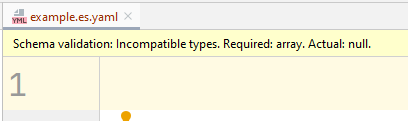
\includegraphics[width=6cm]{images/3.1/Empty} }}%
    \qquad
    \subfloat[\centering Fehlerhafte Eingabe]{{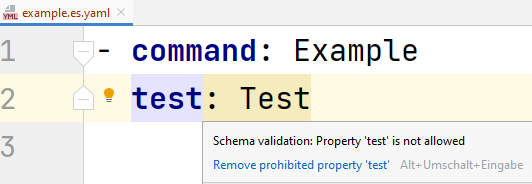
\includegraphics[width=7cm]{images/3.1/fails} }}%
    \caption{Fehleranzeige in IntelliJ}%
    \label{fig:errors-schema}%
\end{figure}

In Abbildung~\ref{fig:errors-schema} ist das Hervorheben von Fehlern in IntelliJ dargestellt, welches durch das JSON-Schema generiert wird.
In Abbildung~\ref{fig:errors-schema}((a)) ist die Datei leer, wodurch die Schema Validierung anschlägt und den Entwickelnden darauf hinweist, dass ein Array, also eine Liste an Elementen, benötigt wird.
Sobald ein Element begonnen wird, wird diese Warnung nicht mehr angezeigt.
Sollte der Entwickelnde wiederum ein Element hinzufügen, welches keinem der definierten Elemente des Schemas entspricht, wird die Meldung aus Abbildung~\ref{fig:errors-schema}((b)) angezeigt.
Da ein Command keine zusätzlichen Attribute/Properties akzeptiert, dennoch eines hinzugefügt wurde, besagt der Fehler, dass es nicht erlaubt ist weitere Attribute hinzuzufügen.

\begin{figure}%
    \centering
    \subfloat[\centering Alle Elemente]{{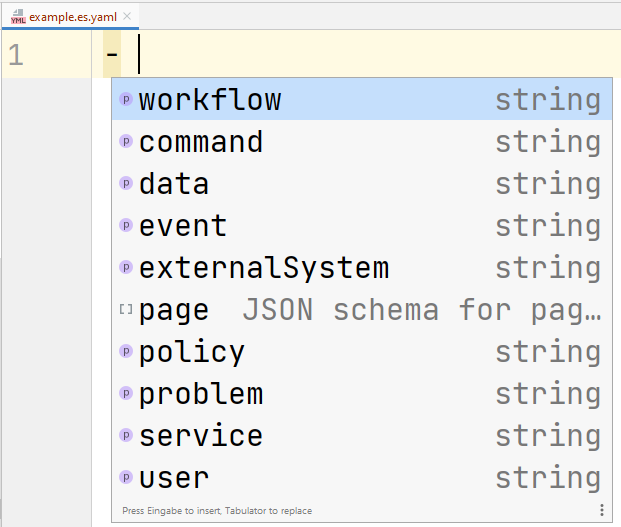
\includegraphics[width=6cm]{images/3.1/all} }}%
    \qquad
    \subfloat[\centering Page Elemente]{{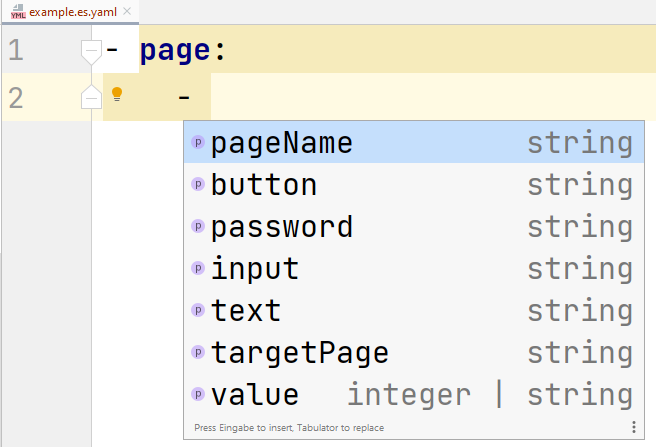
\includegraphics[width=6cm]{images/3.1/page} }}%
    \caption{Autovervollständigung in IntelliJ}%
    \label{fig:completion-schema}%
\end{figure}

Wie zuvor erwähnt ermöglicht ein Schema jedoch nicht nur das Hervorheben von Fehlern, sondern unterstützt den Entwickelnden zusätzlich durch Autovervollständigung.
Dies ist in Abbildung~\ref{fig:completion-schema} dargestellt.
Hierbei werden aufgrund des Kontextes verschiedene Möglichkeiten von zu erstellenden Elementen vorgeschlagen.
Auf oberster Ebene werden alle erlaubten Schlüsselwörter für Elemente angezeigt, dies ist in Abbildung~\ref{fig:completion-schema}((a)) dargestellt.
Hierbei fällt auf, dass die Elemente für eine Page nicht angezeigt werden, dies ist jedoch der Fall, sobald der Kontext dies zulässt.
Während der Entwickelnde ein page-Element definiert, werden wie in Abbildung~\ref{fig:completion-schema}((b)) dargestellt die Schlüsselwörter für Page-Elemente vorgeschlagen.


\subsection{Antlr-Grammatik}\label{subsec:antlr-grammatik}
Da die möglichen Eingaben durch das zuvor beschriebene JSON-Schema bereits verringert wurden, fiel die Wahl der Verarbeitung der YAML-Eingabe auf einen durch Antlr generierten Parser.
Dieser bietet die Möglichkeit, während dem Parsen weitere Aktionen durchzuführen und in dem Fall dieser Anwendung ein Datenmodell aus der Eingabe zu erstellen.
Das Datenmodell wird im folgenden weiterverarbeitet und bietet somit eine Grundlage für die Generierung, auf welche im folgenden Kapitel eingegangen wird.

Wie in Kapitel~\ref{subsubsec:antlr} bereits beschrieben, ist die Grundlage eines Antlr-Parsers die dazugehörige Grammatik, welche nun beleuchtet wird.
Die komplette Grammatik ist im referenzierten fulibWorkflows-Repository im Anhang hinterlegt, in diesem Kapitel werden lediglich Ausschnitte daraus verwendet.
Im Folgenden wird anstatt Zettel zur Beschreibung eines Post-its die englische Übersetzung ``Note'' verwendet, um einen direkten Bezug zu den nachfolgenden Listings herzustellen.

\begin{listing}[!ht]
    \inputminted[firstnumber=5]{antlr-java}{listings/3.1.3/Main.g4}
    \caption{Grammatik für Workflows}
    \label{listing:main-grammar}
\end{listing}

Zuerst wird die grundlegende Struktur einer Datei festgelegt, dies ist durch die drei Regeln in Listing~\ref{listing:main-grammar} dargestellt.
Da eine Datei mehrere Workflows beinhalten kann, ist die oberste Regel in Zeile 5 der Startpunkt des Parsers.
Da als Eingabe eine YAML-Datei ist, heißt die oberste Regel \textit{file} und erfordert mindestens einen~\textit{workflow}.
Ein~\textit{workflow} besteht immer aus einem workflow-Note und beliebig vielen event-Notes, wobei diese immer mit einer Leerzeile von einander getrennt sind.
Die Spezifikation ist aufgrund der YAML-Syntax notwendig.
Ein event-Note ist immer einem von drei Typen zuzuordnen, wobei nach einem Note beliebig viele Leerzeilen folgen können.

\begin{listing}[!ht]
    \inputminted[firstnumber=11]{antlr-java}{listings/3.1.3/Note.g4}
    \caption{Grammatik für Notes}
    \label{listing:note-grammar}
\end{listing}

Die Unterscheidung zwischen normal-/extended-Note, workflow und page erfolgt durch das Schlüsselwort, welches zwischen Bindestrich (\textbf{MINUS}) und Doppelpunkt (\textbf{NAME}) befindet.
Sowohl ein workflow-Note als auch die normal-Notes besitzen lediglich nach dem Doppelpunkt einen Wert, welcher durch \textbf{NAME} gekennzeichnet ist.
Dies ist in Listing~\ref{listing:note-grammar} in Zeile 11 und 13 dargestellt.
Ein extended-Note besitzt neben dem Wert zusätzliche Attribute, welche in einer neuen Zeile beschrieben werden.
Die Anzahl der Attribute ist beliebig, es ist somit erlaubt einen extended-Note ohne weitere Attribute anzugeben.
Die Page ist wie zuvor bereits erwähnt ein Sonderfall, welches sich auch in der Grammatik widerspiegelt.
Dem Schlüsselwort \textit{page} folgt ein gesonderter Doppelpunkt und anschließend eine Liste von neuen Elemente.

\begin{listing}[!ht]
    \inputminted[firstnumber=30]{antlr-java}{listings/3.1.3/Keywords.g4}
    \caption{Schlüsselwörter zum Identifizieren von Notes}
    \label{listing:note-ids}
\end{listing}

Die zuvor erwähnten normal-Notes bestehen wie in Listing~\ref{listing:note-ids} Zeile 30 und 31 dargestellt aus \textit{externalSystem}, \textit{service}, \textit{command}, \textit{policy}, \textit{user} und \textit{problem}.
Diese erhalten lediglich einen Bezeichner und erlauben keine weiteren Attribute.
Zu den extended-Notes zählen lediglich \textit{event} und \textit{data}.
Diese erhalten weitere Attribute, um Daten, welche zwischen Services verschickt werden, darstellen zu können.

\begin{listing}[!ht]
    \inputminted[firstnumber=19]{antlr-java}{listings/3.1.3/Attribute.g4}
    \caption{Grammatik von Attributen}
    \label{listing:attributes}
\end{listing}

Attribute werden eingerückt und enthalten neben einem Bezeichner (\textbf{NAME}) einen dazugehörigen Wert (\textit{value}).
Ein Wert kann entweder ein Text, eine Nummer oder eine Liste sein, wobei eine neue Zeile optional ist.
Die dazugehörigen Regeln sind in Zeile 19 und 21 aus Listing~\ref{listing:attributes} vermerkt.

Wie in Listing~\ref{listing:values} zu sehen ist, ist der akzeptierte Text auf eine feste Menge an verschiedenen Zeichen begrenzt.
Ein Text muss stets mit einem Buchstaben beginnen, ungeachtet ob groß- oder kleingeschrieben.
Darauf können Zahlen, Sonderzeichen und weitere Wörter folgen.
Die Sonderzeichen sind in Zeile 36 genauer beschrieben.

\begin{listing}[!ht]
    \inputminted[firstnumber=36]{antlr-java}{listings/3.1.3/Values.g4}
    \caption{Grammatik von Werten}
    \label{listing:values}
\end{listing}

Eine Nummer kann lediglich eine ganze Zahl sein, führende Nullen sind erlaubt.
Die Möglichkeit als Wert eine Liste angeben zu können, basiert auf der Möglichkeit Objekt- und Klassendiagramme mit fulibWorkflows zu generieren.
Hierzu wurde die Syntax von Java als Grundlage genommen.
Zwischen den Klammern in Zeile 38 befindet sich eine sogenannte Wildcard, welche es erlaubt alle Symbole als Eingabe zu akzeptieren.
Die Klammern erfüllen somit nicht nur den Zweck als Listendarstellung, sondern auch die Begrenzung der Wildcard.
Eine Wildcard für die Eingabe eines Textes zu verwenden war für diese Grammatik aufgrund der Struktur vorerst nicht möglich, da es keine passenden Begrenzungen gab,
welche keine anderen Regeln überschrieben hätte.

\begin{listing}[!ht]
    \inputminted[firstnumber=23]{antlr-java}{listings/3.1.3/Page.g4}
    \caption{Grammatik einer Page}
    \label{listing:page}
\end{listing}

Jeder Page muss ein pageName-Element zugeordnet werden, um sie später referenzieren zu können.
Weiterhin können Pages beliebig viele Elemente beherbergen.
Ein Element kann entweder ein Text, Eingabefeld oder Knopf sein.
Ein Text-Element wird ein Text (\textbf{NAME}) zugeordnet.
Dies ist bei den Eingabefeldern und dem Knopf anders, da diese wie in Kapitel~\ref{subsec:workflow-format} beschrieben zusätzliche
Attribute besitzen können.

Zu dem aus der Grammatik generierten Parser gehört unter anderem ein Interface, welches für diese Grammatik den Namen \textit{FulibWorkflowsListener} trägt.
Um während des Parsens ein Datenmodell aufzubauen, wurde ein eigener Listener implementiert, welcher die Methoden des Interfaces überschreibt.
Für jede Regel aus der Grammatik existiert eine enter- und eine exit-Methode, welche nach enter/exit mit dem Namen der jeweiligen Regel verknüpft ist.
Daraus entstehen Methoden wie zum Beispiel enterPage und exitPage.
In den enter-Methoden werden lediglich neue Objekte angelegt und globale Variablen zurückgesetzt.

\begin{figure}[h]
    \centering
    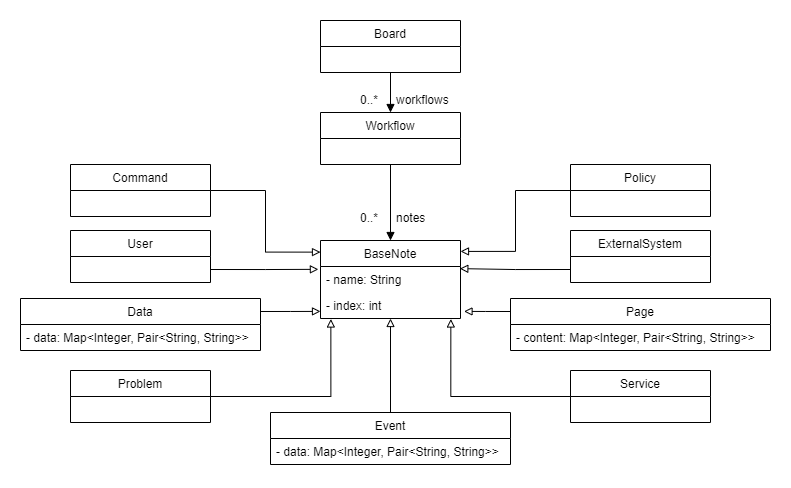
\includegraphics[width=1\textwidth]{images/3.1/classdiagram.drawio}
    \caption{Klassendiagramm fulibWorkflows}
    \label{fig:classdiagram}
\end{figure}

Bevor anhand eines Beispiels die Verwendung einer exit-Methode erläutert wird, ist es notwendig das Datenmodell genauer zu betrachten.
In Abbildung~\ref{fig:classdiagram} ist das Klassendiagramm abgebildet, welches die Struktur eines \ac{ES}-Boards nach dem Parsen der YAML-Eingabe widerspiegelt.
Jeder Note besitzt eine dazugehörige Klasse, welche von BaseNote erbt.
Für jeden Note existiert somit ein Name und ein Index, auf welchen im folgenden Abschnitt eingegangen wird.
Da es im Event Storming ein dazugehöriges \textit{Board} gibt, ist dies ebenfalls eine Klasse, welche alle \textit{workflows} einer Eingabe hält.
Ein Workflow besteht weiterhin aus vielen Notes.
Wie zuvor bereits erläutert, sind Data, Event und Page Sonderfälle unter den Notes, da diese weitere Daten beherbergen.
Daher haben diese Klassen ein Attribut, welches diese Daten organisiert in einer Map hält.
Hierbei wird als key der Index eines Notes verwendet und das value ist ein Pair.
Das Pair beinhaltet den Bezeichner und den dazugehörigen Wert einer zusätzlichen Property eines Notes.

\begin{listing}[!ht]
    \inputminted[firstnumber=106]{java}{listings/3.1.3/ExitPage.java}
    \caption{exitPage-Methode}
    \label{listing:exitpage}
\end{listing}

In Listing~\ref{listing:exitpage} wird ein neues Page-Objekt erstellt.
Bevor jedoch die exitPage-Methode aufgerufen wird, werden alle Elemente der Page in der Variable \textit{noteData} gespeichert.
Diese Elemente werden in der exitElement-Methode hinzugefügt, der Name einer Page wird hingegen in der gesonderten exitPageName-Methode zu \textit{noteData} hinzugefügt.
Zusätzlich zu den Daten eines Notes, wird diesem ein Index gegeben und anschließend zur Liste aller Notes hinzugefügt.
Der Index ist notwendig, um die Reihenfolge von Notes und deren Attributen beizubehalten.



\subsection{Mockups}\label{subsec:mockups}
\todo{this}
Eigenes Datenmodell gebaut.
Daraus die wichtigsten Infos gezogen.
Dank StringTemplates von antlr richtig easy zu bauen.
Gilt für Html als auch Fxml.

\subsection{Generierung dank fulibTools}\label{subsec:generierung-dank-fulibtools}
\todo{this}
FulibTools gibt gute Anbindung an Graphviz, wenn man sowieso schon mit fulib arbeitet.
